% !TeX program = pdflatex
\documentclass[review]{fcs}
\usepackage{layout}
\usepackage{subfig}
\usepackage{hyperref}
\usepackage{graphicx}
\usepackage{booktabs}
\usepackage{multirow}
\usepackage{amssymb}
\usepackage{amsmath}
\usepackage{url}
\usepackage{cite}
\usepackage{enumitem}

% Overleaf compiles from the project root even when this file is the main document.
% Point all graphics explicitly to the official FCS template figure directory.
\graphicspath{{figures/}}

\title{Diagnostics and Infrastructure for Foundation Model-Based Multi-Agent Systems: A Review of the Runtime Stack}

\author[1,+]{Yu~Sun}
\author[2]{Zuodong~Xiang}
\author[3]{Yike~Zhang}
\author[4]{Xinyu~Guan}
\author[5]{Pengcheng~Xu}
\author[3]{Yizirui~Fang}
\author[6]{Zhenhua~Huang}
\author[7]{Hailu~Xu}

\address[1]{School of Engineering and Applied Science, University of Pennsylvania, Philadelphia, PA, United States}
\address[2]{Department of Electrical and Computer Engineering, College of Engineering, University of California, Davis, Davis, CA, United States}
\address[3]{Department of Computer Science, Whiting School of Engineering, Johns Hopkins University, Baltimore, MD, United States}
\address[4]{University of Glasgow, Glasgow, Scotland, United Kingdom}
\address[5]{Department of Computer Science, University of California, Irvine, Irvine, CA, United States}
\address[6]{School of Computer Science, South China Normal University, Guangzhou, Guangdong, China}
\address[7]{Department of Computer Engineering and Computer Science, College of Engineering, California State University, Long Beach, Long Beach, CA, United States}

\corremail{yu.sun@alumni.upenn.edu}
% Yizirui Fang: yizirui.fang@gmail.com
% Zhenhua Huang: huangzhenhua@m.scnu.edu.cn
\fcssetup{
  received = {},
  accepted = {},
  article-id = {},
  first-page = {1},
}

\begin{abstract}
Foundation model-based multi-agent systems are moving into production, yet work on runtime reliability and serving efficiency is still fragmented across diagnostics and infrastructure. This review synthesizes 137 references, 45 systems, and 8 benchmarks through a unified runtime-stack perspective. We organize diagnostics into failure localization, observability, safety, and benchmarks, and infrastructure into memory management, prefix-aware scheduling, cache lifecycle, and power management. The central synthesis is that both layers act on overlapping runtime state but optimize different objectives. Diagnostics benefits from retaining traces, context, and replayable state, whereas serving infrastructure reclaims or compresses state to satisfy memory, latency, and throughput budgets. We term this interaction the \emph{diagnostics--infrastructure retention tension}. We further identify three workload characteristics---sparse activation, invocation distance, and inter-agent memory sharing---that shape agent-aware serving, and use explicit evidence tiers to separate full-text-verified results from abstract-level or contextual evidence. Rather than ranking heterogeneous systems, we derive testable co-design directions: retention-aware eviction, failure-aware scheduling, budgeted observability, and infrastructure-triggered diagnostics. This framing positions runtime state retention as a shared systems resource and clarifies where current multi-agent diagnostics and serving research remain disconnected.

\end{abstract}
\keywords{multi-agent systems; foundation models; diagnostics; observability; serving infrastructure; memory management; scheduling; runtime reliability}

\begin{document}

\section{Introduction}\label{sec:introduction}
Foundation model-based multi-agent systems (MAS), in which multiple Large Language Model (LLM) agents collaborate to solve complex tasks~\cite{metagpt2024, camel2023, chatdev2024}, are increasingly moving from demonstrations toward deployed workflows. A vendor survey reports that 72\% of organizations are actively using or testing multi-agent AI systems~\cite{zapier2025} (Tier-3 vendor data, reported as stated). As systems such as MetaGPT~\cite{metagpt2024}, Internet of Agents~\cite{ioa2025}, and Graph-of-Agents~\cite{graphofagents2026} become more architecturally sophisticated, reliability and efficiency depend on operational layers that are less mature than orchestration itself. We focus on two of them: the \emph{diagnostics layer}, which supports failure localization, observability, and safety, and the \emph{infrastructure layer}, which manages memory, scheduling, and resources for multi-agent workloads.

Existing surveys largely treat these concerns separately. Orchestration frameworks (LangGraph, CrewAI, AutoGen) have received substantial survey attention~\cite{zhu2026orchestration}, as have offline agent evaluation~\cite{evalbenchmark2025, evalagents2026, llmbenchsurvey2025}, safety~\cite{safellmagentsurvey2026, trustworthyagents2025}, AgentOps~\cite{agentopssurvey2025, agentopscsiro2024, architectingops2026}, and single-model serving and latency optimization~\cite{latencysurvey2026}. In our curated corpus, we count 45 systems across our own tables\footnote{Counted across our own system tables: 12 failure-localization methods, 12 observability and safety systems, and 21 infrastructure systems. Benchmarks (8) and comparator surveys (6) are excluded.}. The resulting literature exposes complementary pieces of the runtime stack, but the relationship between the state required for diagnosis and the state managed by serving policies remains under-analyzed.

This review therefore brings the two operational layers into one frame. Table~\ref{tab:surveys} contrasts our scope against six adjacent surveys. General agent surveys~\cite{li2024, abouali2025, wang2026classical, tran2025} cover architectural patterns and collaboration mechanisms; \cite{beyondindiv2026} surveys collaboration and failure but not serving infrastructure; and \cite{li2024} uses ``infrastructure'' for the workflow layer rather than runtime memory, scheduling, cache lifecycle, or power. In the surveyed literature, we did not find a review that jointly organizes runtime diagnostics and multi-agent serving infrastructure while also making the verification depth of quantitative claims explicit.

This is a curated critical review rather than a systematic review. The inclusion boundary, evidence-selection rules, and verification tiers are described in Section~\ref{sec:background}. Quantitative claims used for comparison come from full-text sources; abstract-level results are marked \emph{[a]} and are not used to compute cross-system deltas or rankings. Figure~\ref{fig:overview} illustrates the scope.

\begin{table*}[t]
\centering
\caption{Comparison with existing surveys. $\bullet$ = covered, $\circ$ = not covered. $^a$A 2026 survey of MAS collaboration and failure; it organises failure conceptually and does not catalogue system-level localization methods or cover infrastructure. $^b$A 2024 survey covering workflow and architecture; its ``infrastructure'' is at that level, not multi-agent serving (memory, scheduling, cache lifecycle, power). ``Quant.'' denotes that the survey reports quantitative results for the systems it reviews, at the verification depth described in Section~\ref{sec:background}; it does not imply that those numbers are compared across systems. \textbf{Pub.}: $\checkmark$ = peer-reviewed venue, $\circ$ = preprint, --- = not a publication. Pub.\ records the venue only and is not a quality judgement.}
\label{tab:surveys}
\footnotesize
\setlength{\tabcolsep}{6pt}
\begin{tabular}{@{}llcccccc@{}}
\toprule
\textbf{Survey} & \textbf{Year} & \textbf{Venue} & \textbf{Orch.} & \textbf{Diag.} & \textbf{Infra} & \textbf{Quant.} & \textbf{Pub.} \\
\midrule
Zhu et al. & 2026 & Future Internet & $\bullet$ & $\circ$ & $\circ$ & $\circ$ & $\checkmark$ \\
AgentOps & 2025 & preprint & $\circ$ & $\bullet$ & $\circ$ & $\circ$ & $\circ$ \\
Mohammadi et al. & 2025 & ACM KDD & $\circ$ & $\circ$ & $\circ$ & $\circ$ & $\checkmark$ \\
Latency survey & 2026 & IEEE Access & $\circ$ & $\circ$ & $\bullet$ & $\circ$ & $\checkmark$ \\
Qi et al.$^a$ & 2026 & preprint & $\circ$ & $\bullet$ & $\circ$ & $\circ$ & $\circ$ \\
Li et al.$^b$ & 2024 & Vicinagearth & $\circ$ & $\circ$ & $\circ$ & $\circ$ & $\checkmark$ \\
\textbf{Ours} & 2026 & --- & $\circ$ & $\bullet$ & $\bullet$ & $\bullet$ & --- \\
\bottomrule
\end{tabular}
\end{table*}

\begin{figure*}[t]
\centering
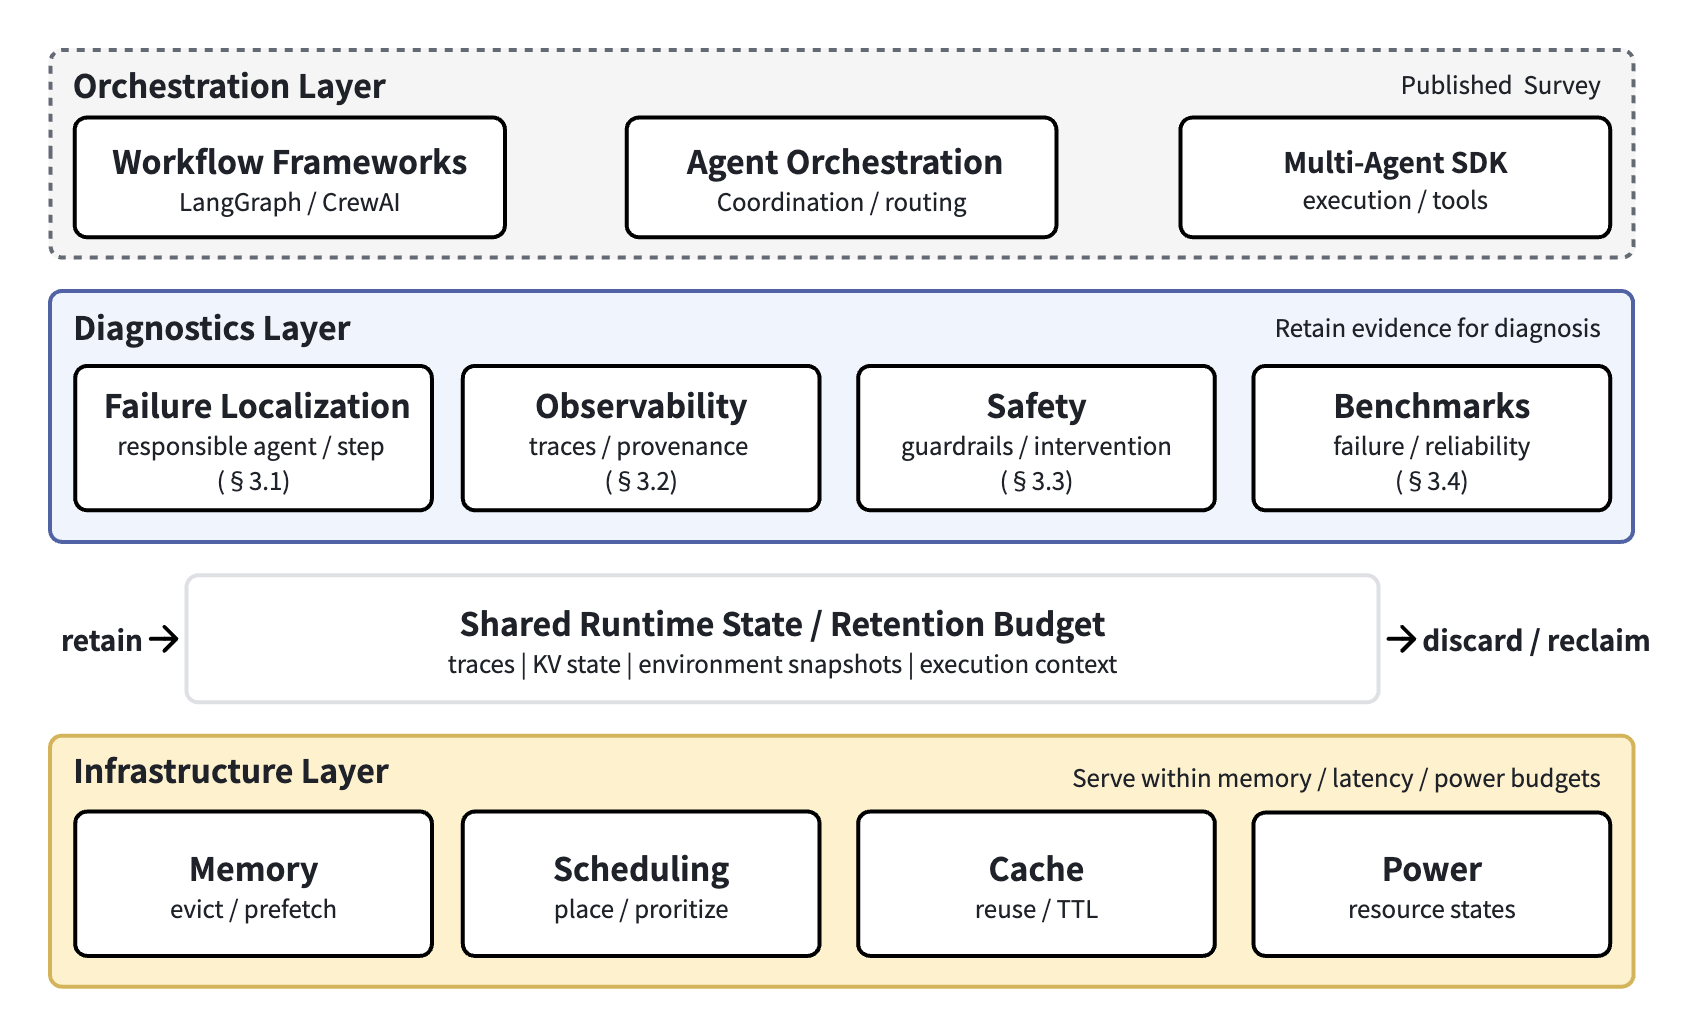
\includegraphics[width=0.75\textwidth]{figure1.png}
\caption{Survey scope: the multi-agent runtime stack. We review the diagnostics layer (Section~\ref{sec:diagnostics}) and the infrastructure layer (Section~\ref{sec:infrastructure}); the orchestration layer is shown for context and is well-covered by existing surveys. The shared runtime-state band marks the retention tension analyzed in Section~\ref{sec:tension}.}
\label{fig:overview}
\end{figure*}

Our contributions are:
\begin{enumerate}
\item \textbf{Diagnostics taxonomy.} We organize multi-agent diagnostics into four subcategories spanning failure localization (Section~\ref{sec:diag_fl}), observability (Section~\ref{sec:diag_obs}), safety (Section~\ref{sec:diag_safety}), and benchmarks (Section~\ref{sec:diag_bench}), covering three failure-localization paradigms (statistical, LLM-guided, RL-trained) and three safety paradigms (topology-based, policy verification, ML-layered).
\item \textbf{Infrastructure challenge analysis.} We identify three multi-agent workload characteristics---sparse activation, invocation distance, and inter-agent memory sharing---that are only partially exposed to general-purpose serving policies, and synthesize application-aware systems spanning memory optimization (ScaleSim, up to 1.74$\times$ speedup~\cite{zhou2026}), prefix-aware scheduling (TokenCake~\cite{tokencake2025}), cache lifecycle (Continuum), and power management (KAIROS).
\item \textbf{Cross-layer tension analysis.} We synthesize a cross-layer retention tension: diagnostics benefits from preserving runtime evidence, while serving infrastructure benefits from reclaiming state under memory and latency budgets. We connect this tension to observed mechanisms in the surveyed systems and derive four co-design opportunities that are made testable in Section~\ref{sec:discussion}.
\end{enumerate}


\section{Background and Review Methodology}\label{sec:background}
A foundation model-based agent operates in a perception--reasoning--action loop, using an LLM to process observations and execute actions such as tool invocations, code execution, and inter-agent communication. The underlying model workloads can also be multimodal: recent systems combine visual, audio, and clinical or platform metadata for domain-specific prediction and governance~\cite{wang-etal-2025-reasoning-enhanced,10.1145/3711896.3737195,xu2026mobifusiondrm}. A multi-agent system (MAS) comprises multiple such agents, as exemplified by MetaGPT~\cite{metagpt2024}, CAMEL~\cite{camel2023}, ChatDev~\cite{chatdev2024}, and IoA~\cite{ioa2025}, operating within a shared environment or communicating to accomplish collective objectives~\cite{li2024, wang2026classical}. Recent multi-agent applications also span reinforcement-learning-enhanced collaborative reasoning and multimodal misinformation detection~\cite{li2026draftrl,li2026retrievalaugmentedfakenews}. MAST~\cite{mast2025} identifies 14 recurring failure patterns in such systems, motivating runtime diagnostics rather than evaluation only at the final task output.

Representation-level adaptation is another adjacent concern: recent speech work studies adversarial attribute obfuscation, accent-controlled editing, and pronunciation representations~\cite{11249000,qu2026partialaccentcontroleditingfrozen,qu2026phonemeawarepronunciationrepresentationsl2english}. These works are not multi-agent infrastructure methods, but they illustrate the heterogeneity of model state and representations that agentic applications may invoke.

Three broad \emph{system properties} recur across the literature reviewed here~\cite{understandingmas2026}: (1)~distributed execution across multiple agents; (2)~inter-agent communication, which creates traces spanning agent boundaries and allows failures to propagate through communication channels~\cite{famas2025, traceelephant2026}; and (3)~inter-agent memory sharing, where prompts, tools, and cached state may be reused across the system. Section~\ref{sec:infra_challenges} derives a serving-side view from these properties and highlights three workload characteristics---sparse activation, invocation distance, and inter-agent memory sharing---that directly affect memory placement, scheduling, and cache policy. This distinction separates general MAS structure from the narrower workload characteristics used in our infrastructure analysis.

\paragraph*{Review scope, selection, and evidence coding.} This article is a curated critical review, not a systematic review. We focus on runtime operational mechanisms for foundation-model agents and MAS, distinct from three well-surveyed areas: orchestration~\cite{zhu2026orchestration}, single-model inference~\cite{kwon2023}, and offline evaluation~\cite{evalbenchmark2025}. For inclusion in the system tables, a work must directly address at least one runtime function in our scope: failure localization, observability/tracing, safety intervention, diagnostic benchmarking, or serving-time memory, scheduling, cache, or power management for agentic workloads. General LLM-serving systems are included when they provide a baseline or mechanism directly reused by agent workloads; orchestration-only frameworks, general agent architectures, and long-term memory representation without serving-time resource management are used only as context. To make the review more reproducible without overstating exhaustiveness, candidate papers were collected iteratively from primary systems papers, adjacent surveys, major peer-reviewed venues, and forward/backward citation tracing. We prioritize work from 2024--2026 because foundation-model multi-agent runtime research is unusually recent, while retaining older serving papers when they define mechanisms directly reused by agentic systems. A paper enters the core system tables only when its runtime role can be identified from the source and mapped to one of the functions above. Because the corpus was not generated by a preregistered database protocol with fixed search strings and PRISMA-style screening, the reported counts should be interpreted as a curated landscape rather than an exhaustive census.

To make the evidential depth of individual claims explicit, we assign cited systems to the following tiers:

\begin{enumerate}
\item \textbf{Tier 1a (full-text verified).} The source was read in full and the specific quantitative claim was located in the body text or a table. These numbers may be compared and quoted when the underlying benchmark and protocol support the comparison.
\item \textbf{Tier 1b (read in full, not page-verified).} The source was read in full and has a confirmed peer-reviewed venue, but the quantitative claim was taken from the published text without being cross-checked against a specific page, table, or figure. These numbers may be quoted with the $^\dagger$ marker but are not used to compute cross-system deltas.
\item \textbf{Tier 2 (abstract-only).} Only the abstract was read; the body was not examined. This applies equally to preprints and venue-published papers whose body we did not read. The claim is reported as stated and marked \emph{[a]}. The distinction from Tier~1b is verification depth, not venue status.
\item \textbf{Tier 3.} Documentation, platform pages, and vendor reports, labelled by source type and used for context only.
\end{enumerate}

Applying this procedure yields \textbf{8 Tier-1 papers across 9 table entries: 5 in Tier~1a} (FAMAS, TrajAudit, Agent Traces, TraceElephant, ScaleSim) and \textbf{3 in Tier~1b} (G-Safeguard at ACL 2025, ShieldAgent at ICML 2025, and AgenTracer at ICLR 2026). RootSE is the benchmark introduced by TrajAudit, so the two rows share one paper. Systems such as RAFFLES, AgentLocate, MultiAgentBench, and Who\&When have confirmed venues but were read at abstract level and therefore remain Tier~2; LlamaFirewall is likewise Tier~2. Throughout the review, publication venue and verification tier are kept separate, and quantitative values from heterogeneous benchmarks are presented as landscape evidence rather than as a global ranking.


\section{Diagnostics}\label{sec:diagnostics}
This section presents our taxonomy of multi-agent diagnostics, organized into four subcategories: failure localization (Section~\ref{sec:diag_fl}), observability (Section~\ref{sec:diag_obs}), safety (Section~\ref{sec:diag_safety}), and benchmarks (Section~\ref{sec:diag_bench}). Figure~\ref{fig:taxonomy} maps the landscape of diagnostic functions and representative systems, whereas Figure~\ref{fig:pipeline} provides a complementary process view showing where tracing, localization, root-cause output, and safety act along execution.

\begin{figure*}[t]
\centering
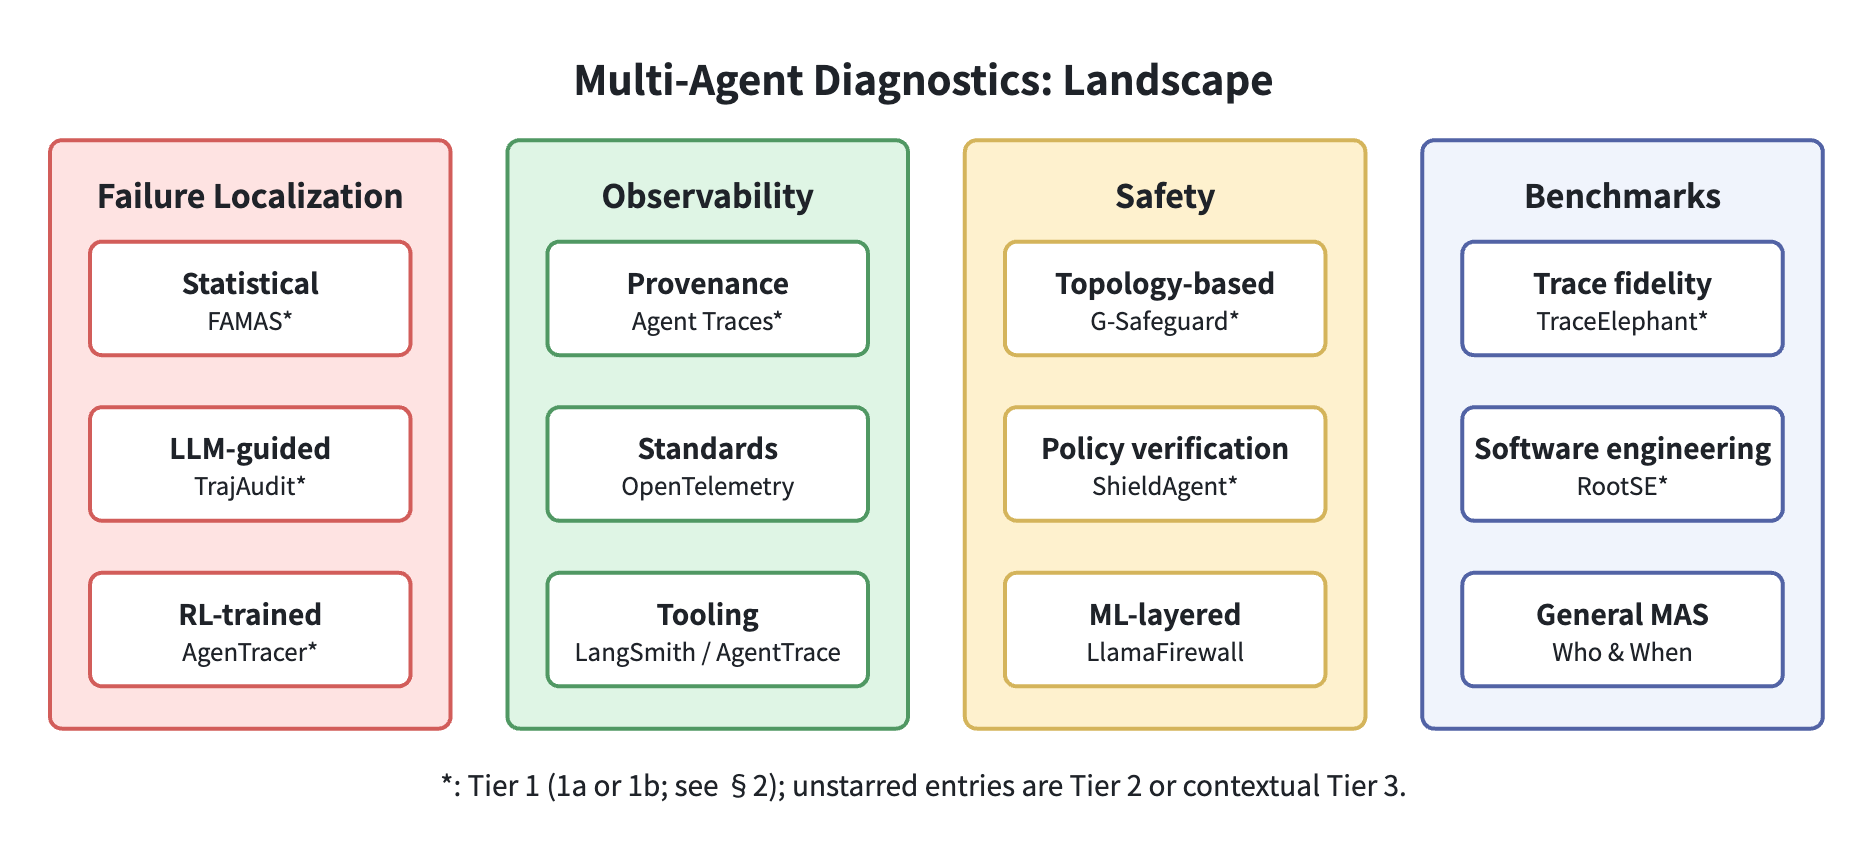
\includegraphics[width=0.75\textwidth]{figure2.png}
\caption{Landscape of multi-agent diagnostics across four subcategories. Stars ($\star$) mark Tier~1 systems (Tier~1a or 1b); unmarked leaves are Tier~2 (abstract-verified) or, for standards and tooling, Tier~3. The tier rule and the 1a/1b split are given in Section~\ref{sec:background}.}
\label{fig:taxonomy}
\end{figure*}

\subsection{Failure Localization}\label{sec:diag_fl}

When a multi-agent system fails, identifying the responsible agent and faulty action remains a central challenge. Our surveyed set contains twelve failure-localization methods from 2024--2026. We group them into three recurring paradigms---statistical, LLM-guided, and RL-trained---that use distinct methodological assumptions and evaluation conventions. These paradigms differ along two axes: \emph{input requirements} (replay-based vs.\ single-execution) and \emph{attribution granularity} (agent-level, step-level, or action-level). Table~\ref{tab:failure_loc} summarizes the landscape.

\paragraph*{Statistical approaches}
These methods apply spectrum-based fault localization (SBFL) to multi-agent traces. FAMAS~\cite{famas2025} replays trajectories $k=20$ times and applies four suspiciousness metrics (action coverage, failure entropy, temporal decay, Kulczynski2), achieving 66\% top-1 action-level accuracy on the 82-failure replayable subset of Who\&When~\cite{famas2025}. Complementary statistical methods extend SBFL without replays: CausalFlow~\cite{flatlogs2026} constructs hierarchical causal graphs (36.2\% step accuracy, abstract-verified) and StepFinder~\cite{stepfinder2026} applies temporal semantic analysis (+10.35pp, abstract-verified). Zero-replay debugging~\cite{zeroreplay2026} eliminates replay overhead entirely through knowledge-based reasoning (abstract-verified).

\paragraph*{LLM-guided approaches}
These treat diagnosis as a reasoning task. Adjacent work on process supervision, structured reasoning supervision, and self-generated rewards similarly studies intermediate or internally generated supervision rather than only final outputs~\cite{liu-etal-2026-ips,jiang-etal-2026-drp,jiang2026scribestructuredmidlevelsupervision,lin2026cec}. TrajAudit~\cite{trajaudit2026} deploys an LLM investigator with Semantic Saliency Folding (SSF, 86--92\% token reduction) and Prior Failure Reasoning (PFR), achieving +24.7pp step-level accuracy on RootSE (93 failures); ablation confirms SSF as critical ($-$11.4\% vs.\ $-$3.5\% for PFR)~\cite{trajaudit2026}. The LLM-guided family has rapidly diversified: AgentRx~\cite{agentrx2026} provides domain-agnostic diagnosis (+23.6pp step, +22.9pp category accuracy), TRAIL~\cite{trail2025} combines trace reasoning with issue localization, RAFFLES~\cite{raffles2026} applies reasoning-based attribution (EACL 2026), and AgentLocate~\cite{agentlocate2026} adds multi-perspective verification. Hierarchical approaches~\cite{hierrerror2025} decompose errors across agent boundaries, while VerifyMAS~\cite{verifymas2026} introduces hypothesis verification for attribution (all abstract-verified).

\paragraph*{RL-trained approaches}
These replace hand-designed metrics with learned attribution. Related data-valuation work uses hierarchical contrastive Shapley values to prioritize samples, illustrating another structured attribution mechanism at the data level rather than the agent-execution level~\cite{xiao2026points}. AgenTracer~\cite{agentracer2026} trains an 8B-parameter failure tracer via reinforcement learning, achieving 69.10\% agent-level accuracy on Who\&When (184 failures), outperforming DeepSeek-R1 by 12.21pp (ICLR 2026)~\cite{agentracer2026}. MASPrism~\cite{masprism2026} takes a lightweight alternative, using a prefill-stage SLM for attribution (abstract-verified).

\paragraph*{Beyond attribution.}
Several methods extend failure localization toward repair and intervention. Related work on counterfactual rollout replay and trajectory-level guidance further illustrates how alternative execution paths or intermediate trajectory structure can provide supervision signals~\cite{li2026counterfactualrolloutreplayforkable,jiang2026bridgingreasoningtrajectoriesonpolicy}.  diagnosis-driven automatic repair~\cite{diagrepair2026} closes the loop from attribution to fix, AgentTether~\cite{agenttether2026} combines graph-guided diagnosis with runtime intervention, and interactive debugging~\cite{interactivedebug2025} enables human-in-the-loop steering (CHI 2025). Additional methods include FALAT~\cite{falat2026} (dependency-guided search), DoVer~\cite{dover2026} (intervention + replay, recovering 18--28\% of failed trials), EAGER~\cite{eager2026} (unsupervised contrastive trace representation), and holistic evaluation frameworks~\cite{holisticeval2026} (all abstract-verified). Meta-evaluation work~\cite{whwhpro2026} has begun assessing the attribution methods themselves, while post-failure reporting benchmarks examine whether tool-using agents can accurately communicate what went wrong after execution~\cite{zhu2026failure}, and the same shift toward online auditing appears in AgentForesight~\cite{agentforesight2026}, which monitors a trajectory while it runs and emits an alarm before the failure surfaces rather than reconstructing it afterwards (abstract-verified).

\begin{table*}[t]
\centering
\caption{Failure localization methods for multi-agent systems. Tier~1 results are from full-text verification, except those marked $^\dagger$, which are venue-published but reported from the published text without page-level cross-verification (Tier~1b); Tier~2 results marked [a] are as reported in source abstracts and are not independently verified. The tier rule and the 1a/1b split are given in Section~\ref{sec:background}. \textbf{Pub.}: $\checkmark$ = peer-reviewed main-track venue, $\circ$ = preprint or workshop paper. --- = not stated in the source. \emph{These numbers come from different benchmarks, protocols, and observability settings; this table is a landscape summary, not a head-to-head comparison (see Section~\ref{sec:tension}).}}
\label{tab:failure_loc}
\scriptsize
\setlength{\tabcolsep}{2pt}
\begin{tabular}{@{}p{0.145\textwidth}p{0.155\textwidth}lp{0.115\textwidth}p{0.125\textwidth}p{0.135\textwidth}cp{0.04\textwidth}@{}}
\toprule
\textbf{System} & \textbf{Approach} & \textbf{Gran.} & \textbf{Bench.} & \textbf{Overhead} & \textbf{Key Result} & \textbf{Tier} & \textbf{Pub.} \\
\midrule
FAMAS & Stat. (SBFL) & Action & Who\&When & 20 replays & 66\% top-1 & 1 & $\circ$ \\
TrajAudit & LLM-guided & Step & RootSE & 86--92\% tok. & +24.7pp & 1 & $\circ$ \\
AgenTracer & RL (8B) & Agent & Who\&When & 8B train & 69.10\% & 1$^\dagger$ & $\checkmark$ \\
AgentRx & LLM-guided & Step & --- & --- & +23.6pp step [a] & 2 & $\circ$ \\
FALAT & Dependency & Step & Who\&When & --- & 46.0\% step [a] & 2 & $\circ$ \\
DoVer & Interv.+Replay & Step & --- & multiple replays & 18--28\% [a] & 2 & $\checkmark$ \\
MASPrism & Prefill SLM & Step & --- & --- & --- [a] & 2 & $\circ$ \\
RAFFLES & Reasoning & Step & Who\&When & --- & --- [a] & 2 & $\checkmark$ \\
AgentLocate & LLM judge & Step & --- & --- & --- [a] & 2 & $\checkmark$ \\
CausalFlow & Stat. (Causal) & Step & --- & --- & 36.2\% [a] & 2 & $\circ$ \\
StepFinder & Temporal sem. & Step & Who\&When & --- & +10.35pp [a] & 2 & $\circ$ \\
EAGER & Contrastive & System & --- & --- & prelim. [a] & 2 & $\circ$ \\
\bottomrule
\end{tabular}
\end{table*}
\vspace{-2pt}
{\footnotesize \emph{Non-comparability.} The ``Key Result'' column aggregates measurements taken on different benchmarks (Who\&When, RootSE, or task-specific sets), under different observability settings (output-only vs.\ full traces), and against different baselines. Methods also differ in what they require at inference time (replay budget, training, token cost). The rows therefore describe a landscape of approaches, not a ranked comparison; no cross-row ranking should be inferred. Pub.\ records the publication venue only and is not a quality judgement.}

\subsection{Observability and Tracing}\label{sec:diag_obs}

Failure localization depends on rich execution traces, yet the multi-agent observability stack remains fragmented across three levels: conceptual models, protocols, and tooling~\cite{aiobsmultilayer2026}. More broadly, recent analyses of reasoning trajectories examine which tokens or intermediate states carry disproportionate learning signal and how reasoning can be evaluated under memorization constraints~\cite{jiang2026rocktokens,jiang-ferraro-2026-beyond}.

At the \emph{conceptual level}, \cite{agenttraces2026} present a seven-dimension provenance taxonomy (trace sources, evidence units, execution units, nine relation types, run-to-token granularity, online/offline timing, interaction context). This taxonomy exposes a key architectural split between post-hoc debugging and runtime enforcement. Complementary taxonomies address observability from an operations perspective~\cite{agentopscsiro2024, architectingops2026, agentsysops2026}, and a multi-layer survey~\cite{aiobsmultilayer2026} proposes a five-layer framework spanning data, model, agent, system, and application observability (all abstract-verified).

At the \emph{protocol level}, the OpenTelemetry GenAI conventions~\cite{opentelemetry2026} provide vendor-neutral attributes (\texttt{gen\_ai.*}) for LLM spans, but semantic interoperability remains limited. AgentTrace~\cite{agenttrace2026} proposes structured logging specifically for agent systems (AAAI 2026 Workshop, abstract-verified), and process mining approaches~\cite{processobserv2025} apply workflow analysis to agent traces (abstract-verified).

At the \emph{tooling level}, a vendor survey reports 89\% observability adoption among enterprises using AI agents~\cite{zapier2025} (Tier-3 vendor data), with LangSmith~\cite{langsmith2026}, Langfuse, and Arize Phoenix as leading platforms. The Insights Generator~\cite{insightsgenerator2026} demonstrates that corpus-level trace mining improves downstream performance by 30.4pp (abstract-verified). Security-focused tooling has also emerged: auditable agent frameworks~\cite{auditableagents2026, secaudit2026} build unified graphs for security auditing, and view-oriented compilers~\cite{viewcompiler2026} enable multi-perspective trace analysis (all abstract-verified).

Table~\ref{tab:obs_safety} summarizes the observability and safety landscape.

\begin{table*}[t]
\centering
\caption{Observability, tracing, and safety systems. \textbf{Pub.}: $\checkmark$ = peer-reviewed main-track venue, $\circ$ = preprint, workshop paper, or no confirmed venue, --- = documentation or platform (not a publication). Pub.\ records the venue only and is not a quality judgement.}
\label{tab:obs_safety}
\footnotesize
\setlength{\tabcolsep}{5pt}
\begin{tabular}{@{}llccc@{}}
\toprule
\textbf{System} & \textbf{Category} & \textbf{Open} & \textbf{Tier} & \textbf{Pub.} \\
\midrule
\multicolumn{5}{l}{\emph{Observability \& Tracing}} \\
Agent Traces & Taxonomy & --- & 1 & $\circ$ \\
OTel GenAI & Standard & \checkmark & 3 & --- \\
AgentTrace & Structured log & --- & 2 & $\circ$ \\
LangSmith & Platform & --- & 3 & --- \\
Insights Gen. & Diagnostic & --- & 2 & $\circ$ \\
\midrule
\multicolumn{5}{l}{\emph{Safety \& Reliability}} \\
G-Safeguard & Topology GNN & --- & 1$^\dagger$ & $\checkmark$ \\
ShieldAgent & Policy verif. & --- & 1$^\dagger$ & $\checkmark$ \\
LlamaFirewall & ML-layered & \checkmark & 2 & $\circ$ \\
SAIGuard & Proactive MAS & --- & 2 & $\circ$ \\
AGrail & Lifelong guard & --- & 2 & $\circ$ \\
AgentDoG & Alignment & --- & 2 & $\circ$ \\
ReGuard & Reactive & --- & 2 & $\circ$ \\
\bottomrule
\end{tabular}
\par\vspace{2pt}{\footnotesize $^\dagger$Venue-published; not page-level verified.}
\end{table*}

\subsection{Safety and Reliability}\label{sec:diag_safety}

Multi-agent safety poses a distinct challenge: attacks propagate through inter-agent communication, so a single compromised agent can corrupt downstream outputs~\cite{safellmagentsurvey2026, trustworthyagents2025}. Recent surveys identify this cross-agent propagation as the defining difference from single-agent safety~\cite{fullstacksafety2025}. Three paradigms have emerged, each at a different abstraction level. We follow the literature's convention of treating safety as a diagnostic subcategory; as Section~\ref{sec:discussion} argues, this placement is contestable, because a guardrail must both inspect state and act on the serving path.

\emph{Topology-based} approaches exploit the communication graph. G-Safeguard~\cite{gsafeguard2025} uses a GNN to detect anomalies on the multi-agent utterance graph and applies topological intervention, recovering over 40\% of the performance lost to prompt injection (ACL 2025; Tier 1b). SAIGuard~\cite{saiguard2026} extends this to communication-state simulation for proactive defense, SentinelAgent~\cite{sentinelagent2025} detects node-, edge-, and path-level anomalies on a typed execution graph, and BlindGuard~\cite{blindguard2025} performs the same detection without attack labels by training on normal-only interaction data (all abstract-verified). This graph-level reasoning is particularly salient in multi-agent settings because failures can propagate across inter-agent communication edges.

\emph{Policy-reasoning guardrails} verify another agent's action trajectory against explicit safety policies. ShieldAgent~\cite{shieldagent2025} is a single guardrail agent that extracts verifiable rules from policy documents and checks each proposed action against them, reporting 90.1\% recall of violated rules while using 64.7\% fewer API queries and 58.2\% less inference time than prior approaches (ICML 2025; Tier~1b). \cite{probabilisticarchitecture2026} provide a theoretical foundation via a three-layer probabilistic architecture, and VeriGuard~\cite{veriguard2025} applies verified code generation for safety-critical agents. The Swiss Cheese model~\cite{swisscheese2025} offers a complementary defense-in-depth framework (all abstract-verified).

\emph{ML-layered} defenses stack classifiers. LlamaFirewall~\cite{llamafirewall2025} layers PromptGuard2 (AUC 0.98) with an alignment verifier, reducing attack success from 17.6\% to 1.75\%. AGrail~\cite{agrail2025} introduces lifelong adaptive guardrails that evolve with agent deployment (abstract-verified), and GuardAgent~\cite{guardagent2024} enables knowledge-based guardrail reasoning (abstract-verified).

Complementary systems span pre-execution alignment (AgentDoG~\cite{agentdog2026}), control-theoretic recovery (ReGuard~\cite{pandya2025}), automated auditing (AgentAuditor~\cite{agentauditor2025}, NeurIPS 2025), and admission control for privileged LLM agents~\cite{zhu2026leaseguard}. Safety benchmarks include GuardianAgentBench~\cite{guardianagentbench2026} (580 scenarios), OSGuard~\cite{osguard2026} (2.7\% FPR), Agent-SafetyBench~\cite{agentsafetybench2024}, and AgentHarm~\cite{agentharm2024} (all abstract-verified).

\subsection{Benchmarks}\label{sec:diag_bench}

Progress in diagnostics depends on benchmarks varying in failure coverage, trace fidelity, and evaluation scope. Table~\ref{tab:benchmarks} summarizes the landscape.

The highest-fidelity benchmark is TraceElephant~\cite{traceelephant2026}: 220 failures from three production systems with full observability. At the \emph{agent} level, complete traces raise attribution accuracy from 51\% for output-only logs to 62.2\% (+11.2pp, a 22\% relative gain), both under the same All-at-Once protocol. At the \emph{step} level, the same comparison raises accuracy from 16\% to 28.1\% (+12.1pp, a 76\% relative gain), i.e.\ step-level attribution is substantially more sensitive to missing information than agent-level attribution~\cite{traceelephant2026}. Who\&When~\cite{whenwhen2025} provides 184 failures from 127 multi-agent systems as the first dedicated failure attribution benchmark, now with a meta-evaluation extension~\cite{whwhpro2026} (abstract-verified). Domain-specific, RootSE~\cite{trajaudit2026} offers 93 SWE-bench failures with step-level annotations.

Beyond failure attribution, ReliabilityBench~\cite{reliabilitybench2026} reveals that pass@1 overestimates reliability by 20--40\% (abstract-verified), BenchGuard~\cite{benchguard2026} audits benchmark quality (abstract-verified), and MultiAgentBench~\cite{multiagentbench2025} evaluates multi-agent collaboration (ACL 2025, abstract-verified). Safety-specific benchmarks include Agent-SafetyBench~\cite{agentsafetybench2024}, AgentHarm~\cite{agentharm2024}, Agent Security Bench~\cite{asb2025} (ICLR 2025, which reports attack success above 84\% with existing defenses barely effective), and TAMAS~\cite{tamas2026} (ACL 2026, covering Byzantine, colluding, and contradicting agents) (all abstract-verified). A unified capabilities framework~\cite{unifiedcapab2026} and a benchmarking survey~\cite{evalbenchmark2025} address the meta-question of what benchmarks should measure.

\begin{table*}[t]
\centering
\caption{Diagnostics and safety benchmarks. \textbf{Pub.}: $\checkmark$ = peer-reviewed venue, $\circ$ = preprint / no confirmed venue. Pub.\ records the venue only and is not a quality judgement.}
\label{tab:benchmarks}
\footnotesize
\setlength{\tabcolsep}{5pt}
\begin{tabular}{@{}lccccc@{}}
\toprule
\textbf{Benchmark} & \textbf{Scale} & \textbf{Traces} & \textbf{Domain} & \textbf{Tier} & \textbf{Pub.} \\
\midrule
TraceElephant & 220 & Full & Multi & 1 & $\circ$ \\
Who\&When & 184 & Output & Multi & 2 & $\checkmark$ \\
RootSE & 93 & Full & SWE & 1 & $\circ$ \\
MultiAgentBench & --- & --- & Collab & 2 & $\checkmark$ \\
Agent-SafetyBench & --- & --- & Safety & 2 & $\circ$ \\
AgentHarm & --- & --- & Safety & 2 & $\circ$ \\
ReliabilityBench & --- & --- & Reliab. & 2 & $\circ$ \\
BenchGuard & --- & --- & Meta & 2 & $\circ$ \\
\bottomrule
\end{tabular}
\end{table*}

Among the benchmarks surveyed here, none evaluates diagnostics--infrastructure interaction: how diagnostic overhead affects serving performance, or how retention and serving policies affect diagnostic fidelity.

\paragraph*{Diagnostics synthesis.} Across the four diagnostic subcategories, the common dependency is retained execution evidence: localization methods require traces or replays, observability determines what evidence exists, and safety mechanisms must inspect enough context to intervene. The literature is broad but methodologically heterogeneous, so the taxonomy is most useful for comparing assumptions---trace fidelity, replay budget, granularity, and intervention timing---rather than headline accuracy across rows. This shared dependence on runtime evidence motivates the retention analysis in Section~\ref{sec:tension}.

\begin{figure*}[t]
\centering
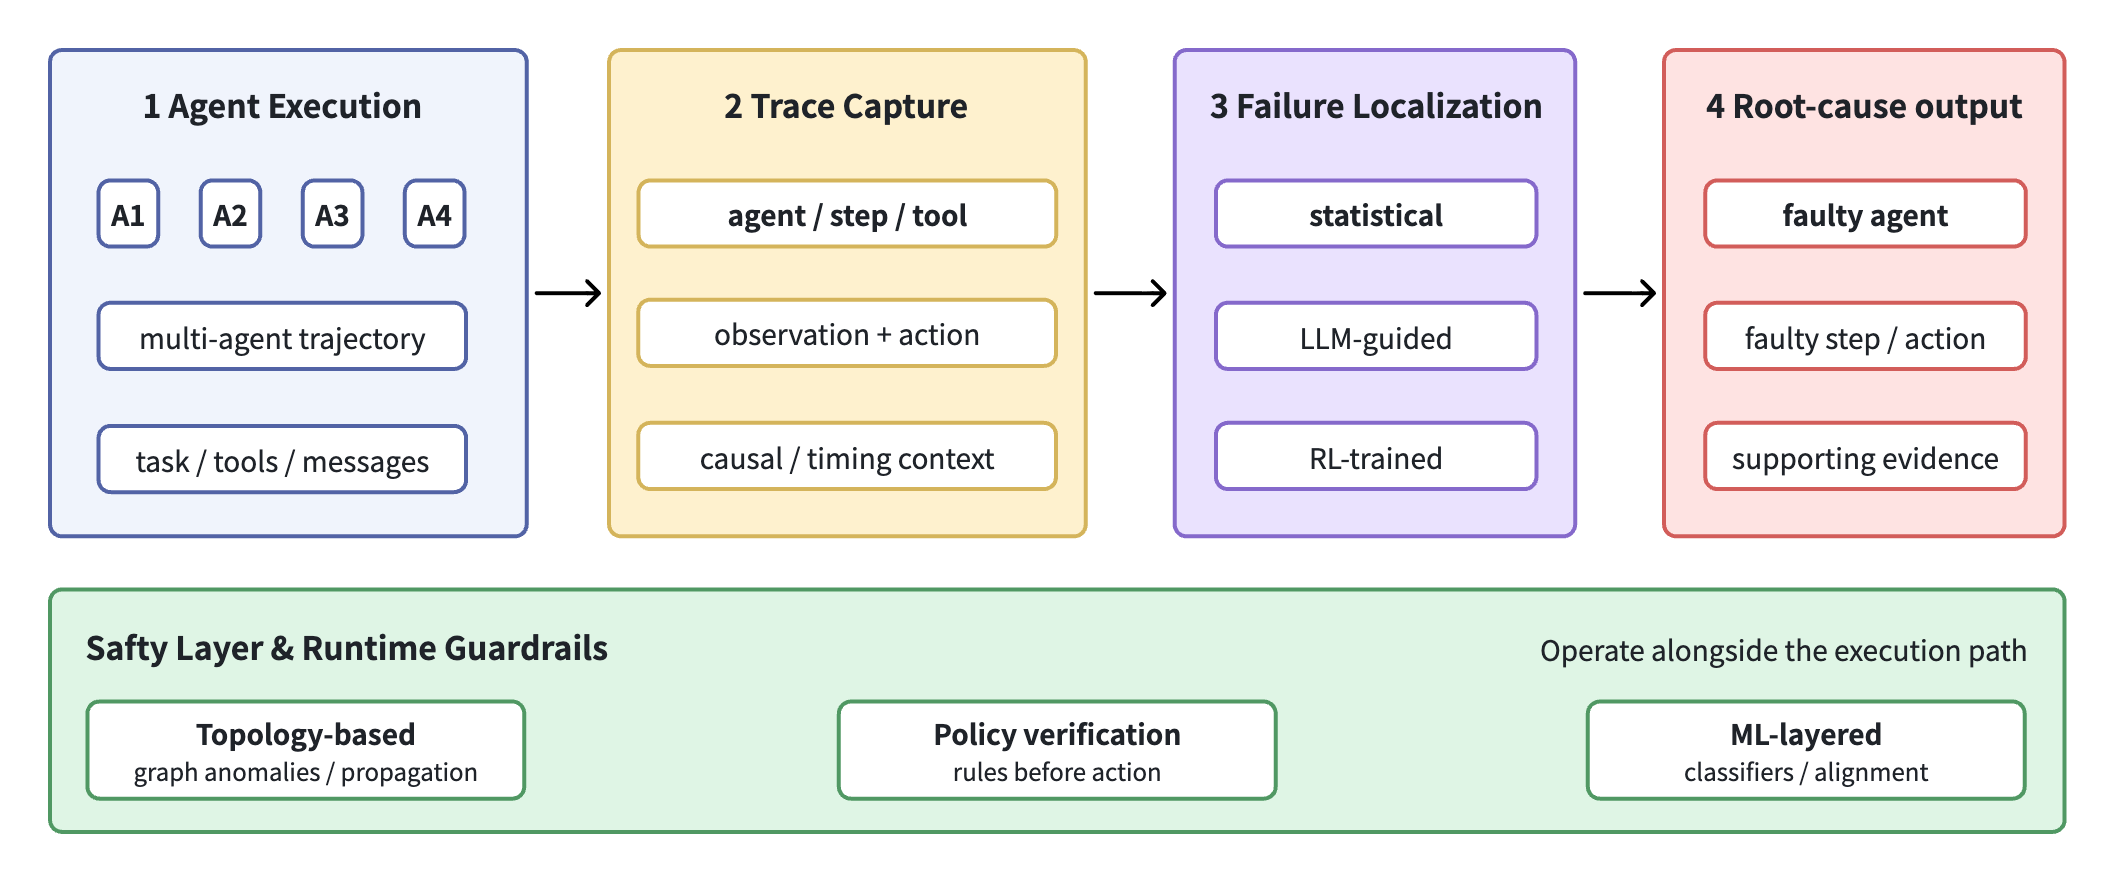
\includegraphics[width=0.9\textwidth]{figure3.png}
\caption{Process view of multi-agent diagnostics. Execution traces are collected through observability infrastructure, then processed through failure localization to produce root-cause attribution, while safety mechanisms may operate continuously alongside execution. This figure complements the landscape in Figure~\ref{fig:taxonomy}: it shows when diagnostic functions act rather than reclassifying the systems.}
\label{fig:pipeline}
\end{figure*}


\section{Infrastructure}\label{sec:infrastructure}
Most LLM serving systems were designed around request-level inference and expose only part of the structure available in multi-agent workloads. We identify three multi-agent serving challenges (Section~\ref{sec:infra_challenges}), analyze application-aware systems that exploit them (Section~\ref{sec:infra_scalesim}), and map the broader infrastructure landscape (Section~\ref{sec:infra_landscape}).

\subsection{Multi-Agent Serving Challenges}\label{sec:infra_challenges}

Single-model serving systems (vLLM~\cite{kwon2023}, SGLang~\cite{sglang2024}, DistServe~\cite{distserve2024}) primarily optimize request execution. Energy-efficient retrieval-augmented generation on resource-constrained devices provides a complementary efficiency perspective outside the multi-agent serving setting~\cite{cheng2026toward}. Peer-reviewed serving work has also begun to expose application structure: Parrot~\cite{parrot2024} passes an application-level dependency graph (semantic variables) to the scheduler, Preble~\cite{preble2025} optimizes distributed prompt sharing, Sarathi-Serve~\cite{sarathi2024} introduces chunked prefill, InferCept~\cite{infercept2024} retains KV state across tool-call interruptions, and S-LoRA~\cite{slora2024} and dLoRA~\cite{dlora2024} serve many concurrent adapters. These systems approach agentic serving from the general side; we return to how they differ from agent-native designs in Section~\ref{sec:tension}. We highlight three workload properties that are particularly relevant to multi-agent execution (cf. the broader KV-cache management landscape surveyed by \cite{kvcachesurvey2026}).

\textbf{Sparse activation.} Only a fraction of agents invoke the LLM at any moment: a 1,000-agent simulation may have fewer than 10 actively generating tokens~\cite{zhou2026}. Under such workloads, keeping all agent state on the fastest memory tier can waste scarce accelerator memory.

\textbf{Invocation distance.} Many workloads have structured activation patterns such as sequential queues, event-driven messaging, and dependency graphs. The temporal gap before an agent's next call, termed \emph{invocation distance}~\cite{zhou2026}, can be estimated from application semantics in structured workloads but is not generally visible to request-level schedulers.

\textbf{Inter-agent memory sharing.} Agents may share context such as system prompts, environment descriptions, and tool schemas, and general serving systems already reuse such prefixes once they appear: SGLang's RadixAttention and vLLM's automatic prefix caching both do this. The additional opportunity in agentic systems is to use application-level future call structure (dependency graphs, message queues, or execution order) to guide prefetching and eviction. TokenDance~\cite{tokendance2026} proposes collective KV-cache sharing across agents, DroidSpeak~\cite{droidspeak2024} enables cache reuse across different model variants, KVFlow~\cite{kvflow2025} exploits an agent step graph to evict workflow-aware and prefetch ahead of the predicted next call, and KVCOMM~\cite{kvcomm2025} aligns cache offsets across divergent per-agent prefixes so that cross-agent reuse survives the prefix change (all abstract-verified). Persistent agent-memory systems (for example A-MEM and the Mesh Memory Protocol) address a related but distinct problem, long-term memory representation rather than serving-time cache reuse, and are outside our scope. Concept-graph memory for vision--language adaptation provides another example of structured long-term representation, distinct from serving-time KV-cache management~\cite{zhou2026comem}.

\subsection{Application-Aware Serving}\label{sec:infra_scalesim}

Recent systems show how multi-agent or agentic workload structure can be exploited across four optimization axes: memory optimization, prefix-aware scheduling, cache lifecycle, and power management.

\paragraph*{Memory optimization via invocation distance.}
ScaleSim~\cite{zhou2026} introduces invocation distance as a first-class scheduling primitive. Two mechanisms exploit predictions: \emph{proactive prefetching} loads agent states before they are needed, and \emph{distance-aware eviction} replaces LRU with future-need predictions, achieving up to 1.74$\times$ speedup over SGLang~\cite{zhou2026}. Its limitation is predictable simulation workloads; interactive agents are less structured.

\paragraph*{Prefix-aware scheduling.}
TokenCake~\cite{tokencake2025} and TOPAS~\cite{topas2026} exploit shared prefixes across agents. TokenCake reports 47\% latency reduction and 16.9\% memory improvement over vLLM (abstract-verified). These figures are reported as stated by the source and are not comparable to ScaleSim's verified up to 1.74$\times$, since the two measure different quantities on different workloads. ForkKV~\cite{forkkv2026} introduces copy-on-write semantics for disaggregated KV caches, which allows efficient prefix sharing without redundant copies (abstract-verified). Prediction-based KV-cache management~\cite{predkvcache2026} applies learned policies to anticipate cache needs (abstract-verified).

\paragraph*{Cache lifecycle and power management.}
Continuum~\cite{continuum2025} introduces KV cache TTL policies for interactive tool-calling agents with unpredictable pauses (abstract-verified). KAIROS~\cite{kairos2026} introduces context-aware power management adapting GPU power states to agentic workload phases (abstract-verified). Together with ScaleSim and TokenCake, these systems illustrate that multi-agent serving exposes optimization opportunities along multiple axes; in the surveyed set, coverage remains partial rather than end-to-end.

\subsection{System Landscape}\label{sec:infra_landscape}

Table~\ref{tab:infrastructure} summarizes the broader infrastructure landscape. Beyond the application-aware systems above, infrastructure-aware orchestration (INFRAMIND~\cite{inframind2026}) bridges scheduling and placement decisions (abstract-verified). Autellix~\cite{autellix2025} provides a dedicated serving engine for LLM agents (abstract-verified), and policy-driven runtime layers~\cite{policyruntime2026} and persistent agent memory~\cite{agentmemory2026} address the system-level integration gap. Baseline serving (vLLM~\cite{kwon2023}, SGLang~\cite{sglang2024}, FlexGen~\cite{flexgen2023}) and disaggregated approaches (DistServe~\cite{distserve2024}) provide the foundation, and Mooncake~\cite{mooncake2025} extends disaggregation to a cluster-wide KV-cache pool, reporting large capacity gains under SLO on production Kimi traffic (abstract-verified). An IEEE survey~\cite{latencysurvey2026} proposes a four-layer latency optimization taxonomy, and the model-native computing architecture~\cite{modelnative2026} reconsiders the full system stack for foundation model workloads (both abstract-verified).

\paragraph*{Synthesis.} The recurring pattern is that agent-specific infrastructure gains come from exposing structure that request-level serving would otherwise treat as opaque: future invocation order, shared prefixes, idle phases, and cache lifetime. Evidence remains uneven---ScaleSim is our full-text case study, while most other agent-specific systems are abstract-verified---so we treat the four axes as a map of design directions rather than a performance ranking. Within the surveyed set, we did not identify a system that jointly optimizes all four axes or uses diagnostic signals as a first-class serving input; this motivates the cross-layer analysis in Section~\ref{sec:tension}.

\begin{table*}[t]
\centering
\caption{Multi-agent infrastructure systems. [a] = abstract-verified. \textbf{Pub.}: $\checkmark$ = peer-reviewed venue, $\circ$ = preprint / no confirmed venue, --- = no publication (platform/docs). Pub.\ records the venue only and is not a quality judgement.}
\label{tab:infrastructure}
\footnotesize
\setlength{\tabcolsep}{5pt}
\begin{tabular}{@{}llcc@{}}
\toprule
\textbf{System} & \textbf{Category} & \textbf{Tier} & \textbf{Pub.} \\
\midrule
ScaleSim & Memory mgmt. & 1 & $\circ$ \\
TokenCake & KV-cache sched. & 2 & $\circ$ \\
TOPAS & Prefix-aware & 2 & $\circ$ \\
KVFlow & Prefix KV-cache & 2 & $\circ$ \\
ForkKV & Copy-on-write KV & 2 & $\circ$ \\
Continuum & Cache lifecycle & 2 & $\circ$ \\
KAIROS & Power mgmt. & 2 & $\circ$ \\
TokenDance & KV sharing & 2 & $\circ$ \\
DroidSpeak & Cross-LLM KV & 2 & $\circ$ \\
Autellix & Agent serving & 2 & $\circ$ \\
INFRAMIND & Infra-aware & 2 & $\circ$ \\
KVCOMM & Cross-agent KV & 2 & $\checkmark$ \\
Mooncake & KV-cache pool & 2 & $\checkmark$ \\
Parrot & App-level DAG & 2 & $\checkmark$ \\
InferCept & KV intercept & 2 & $\checkmark$ \\
Sarathi-Serve & Chunked prefill & 2 & $\checkmark$ \\
Preble & Prompt sharing & 2 & $\checkmark$ \\
S-LoRA & Multi-adapter & 2 & $\checkmark$ \\
dLoRA & Adapter orch. & 2 & $\checkmark$ \\
vLLM & Baseline serving & 2 & $\checkmark$ \\
SGLang & Baseline serving & 2 & $\checkmark$ \\
\bottomrule
\end{tabular}
\end{table*}

\begin{figure*}[t]
\centering
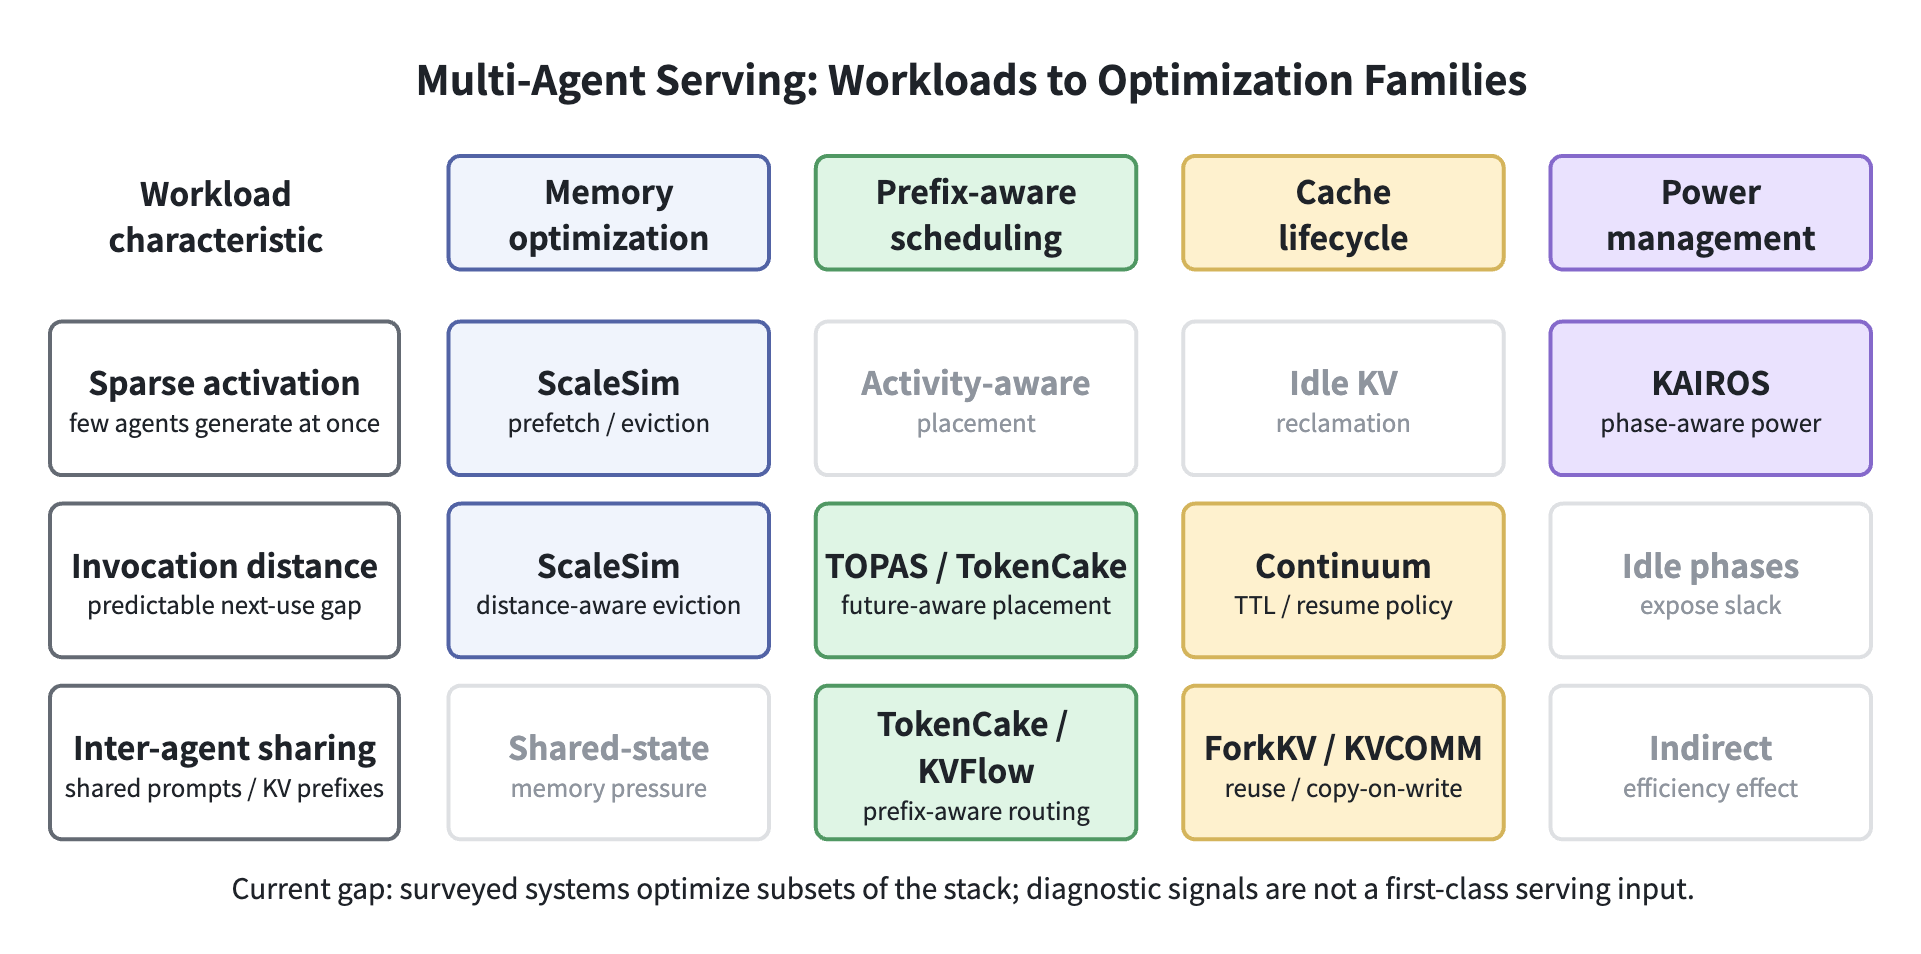
\includegraphics[width=0.8\textwidth]{figure4.png}
\caption{Multi-agent serving challenges and optimization axes. Three workload characteristics---sparse activation, invocation distance, and inter-agent memory sharing---motivate four families of application-aware systems spanning memory optimization, prefix-aware scheduling, cache lifecycle, and power management. The figure maps coverage in the surveyed set; it is not a claim that one system should optimize every axis simultaneously.}
\label{fig:infra_axes}
\end{figure*}


\section{Diagnostics--Infrastructure Retention Tension}\label{sec:tension}
The two layers surveyed so far are usually discussed as independent engineering problems, but both place requirements on the same runtime state. Diagnostics benefits from state being \emph{retained} long enough to explain a failure; serving infrastructure benefits from reclaiming state when doing so improves memory, latency, or throughput. The organising axis is therefore \emph{retention}, not simply timing: a serving policy determines what runtime evidence remains available, and diagnosis---online or after the fact---must work from what survives. In the surveyed systems, retention decisions are made locally inside the serving or diagnostic component rather than negotiated across layers.

TraceElephant provides the clearest measured example of why retained evidence matters. Under the same All-at-Once attribution protocol, complete traces raise agent-level accuracy from 51\% to 62.2\%, and step-level accuracy from 16\% to 28.1\% (a 76\% relative gain)~\cite{traceelephant2026}. The comparison does not by itself establish why a production system might retain less information, but it quantifies the diagnostic consequence of reduced observability. This is the empirical anchor for treating trace retention as a cross-layer resource rather than assuming that diagnostic fidelity is independent of serving-state policy.

\begin{figure*}[t]
\centering
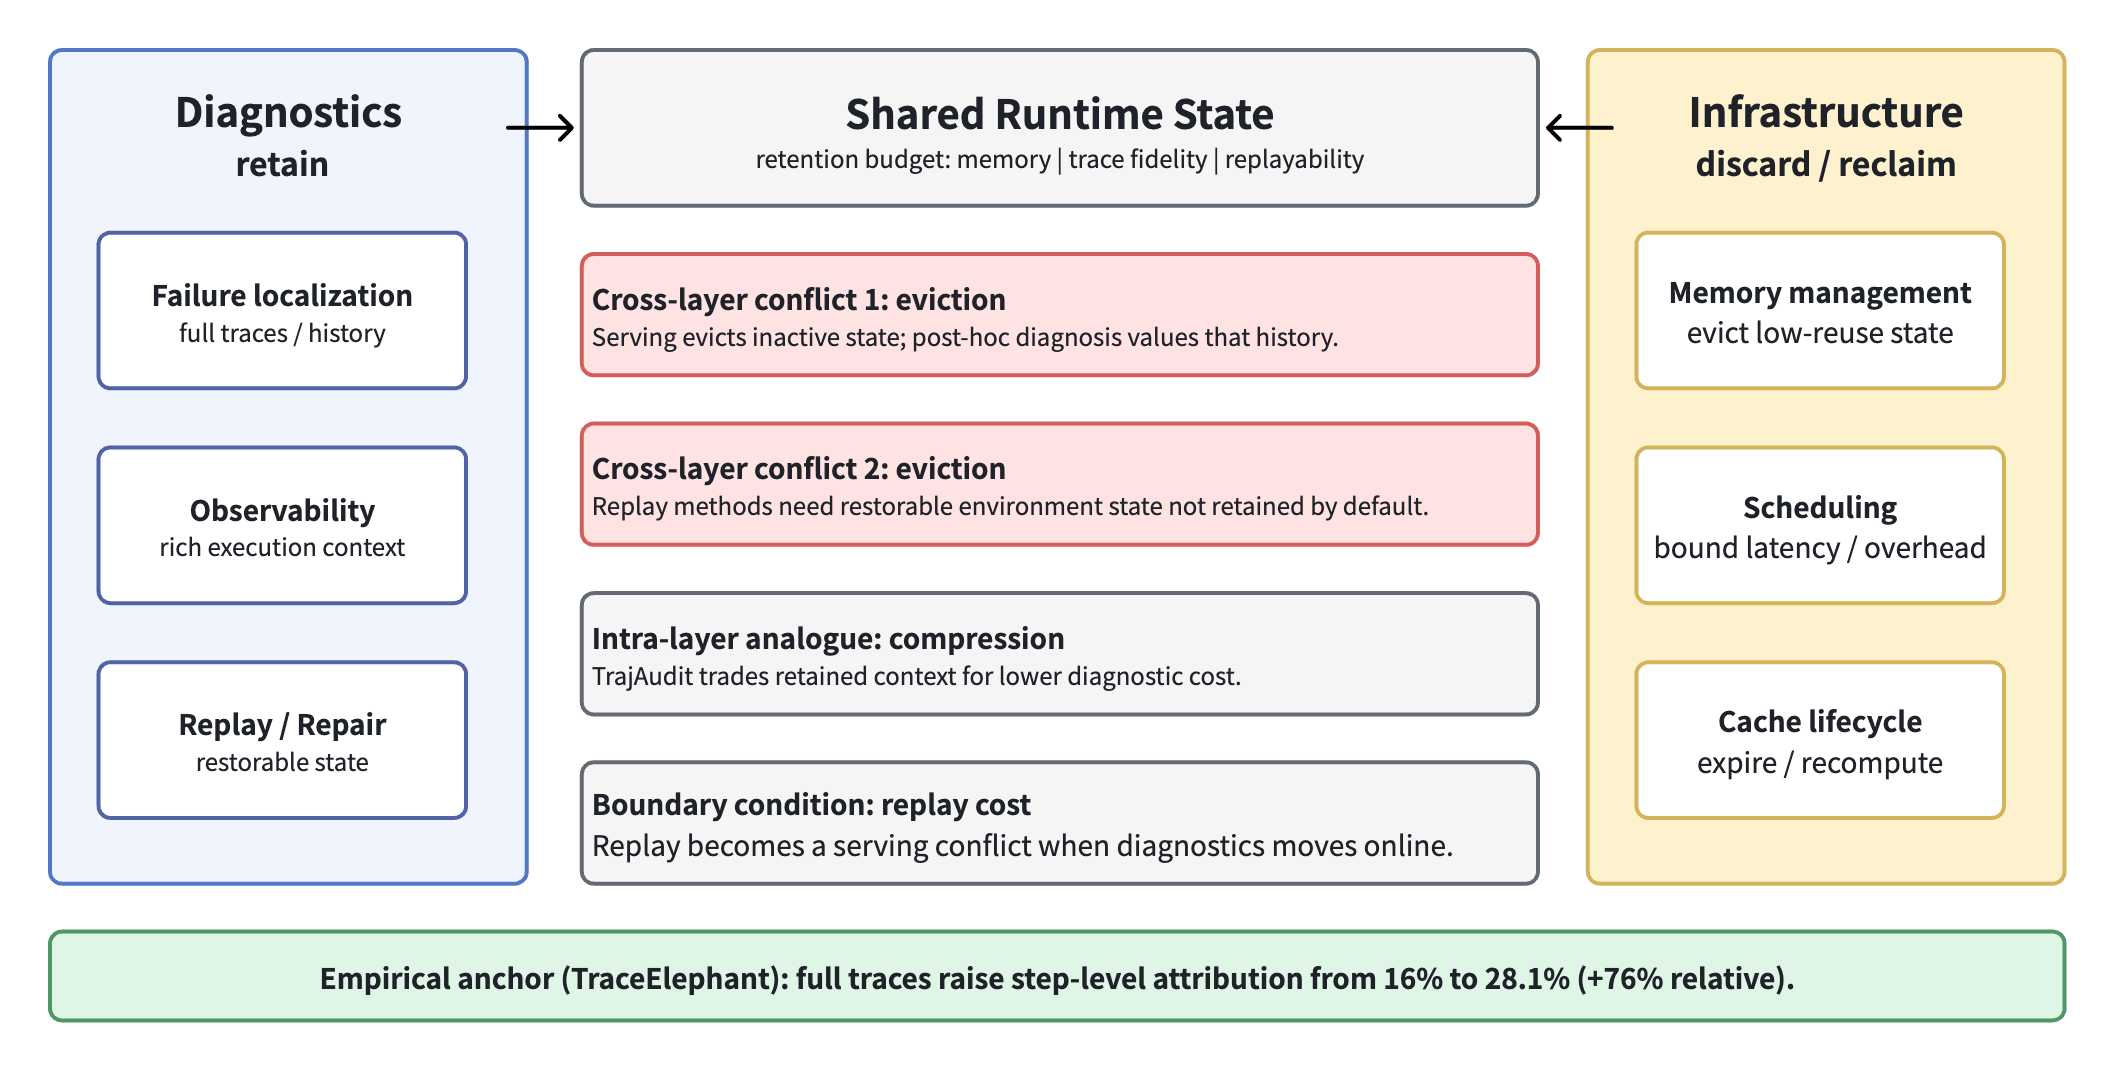
\includegraphics[width=0.8\textwidth]{figure5.png}
\caption{The diagnostics--infrastructure retention tension. The diagnostics layer (left) benefits from retaining runtime evidence for failure explanation, while the infrastructure layer (right) reclaims state under memory, latency, and throughput budgets. The centre summarizes two cross-layer conflict mechanisms, one intra-layer analogue, and one boundary condition. Among the surveyed systems, none manages retention as an explicit cross-layer budget.}
\label{fig:tension}
\end{figure*}

We call this the diagnostics--infrastructure retention tension. It is a trade-off, not a claim that every infrastructure optimization necessarily harms diagnosis: the two layers optimize different objectives over overlapping runtime objects, and the conflict appears when reclaiming or compressing those objects removes evidence needed later. Two cross-layer mechanisms make the issue concrete; a third instance shows the same shape within the diagnostic layer itself; and a fourth marks where the conflict would become acute for online diagnosis.

\emph{Swapping state off the fast path.} ScaleSim's distance-aware eviction~\cite{zhou2026} prioritizes agent states with long invocation distance for movement off the fastest memory tier. From a diagnostic perspective, those inactive states can still contain history useful for later reconstruction. ScaleSim does not delete the state by definition; the relevant cross-layer question is whether moved state, associated KV cache, and related execution context remain available long enough for diagnosis or are later reclaimed or recomputed. The surveyed serving policy optimizes reuse and memory pressure, not diagnostic value, which exposes the difference in objectives without implying that eviction always destroys evidence.

\emph{Environment snapshots are not a first-class serving primitive.} Replay-based attribution needs more than a text trace. FAMAS~\cite{famas2025} re-executes a failed task $k=20$ times and expects the environment to reach comparable states, and DoVer~\cite{dover2026} intervenes mid-trajectory and reruns from the intervention point, which requires the environment to be restorable. The serving systems surveyed here do not expose environment-snapshot retention as a diagnostic primitive. Consequently, replay-based methods are typically evaluated on fixed corpora or reconstructable environments rather than under a live serving policy with an explicit snapshot budget.

\emph{The diagnostic layer has an isomorphic tradeoff internally.} TrajAudit's Semantic Saliency Folding~\cite{trajaudit2026} compresses 86--92\% of observations into placeholders to fit the model's context window. This is the diagnostician's own retention decision, with more context potentially supporting attribution and compression lowering cost. It is not a cross-layer conflict, but it shows that evidence retention already appears as a cost--fidelity trade-off inside diagnostics.

\emph{Replay is a serving cost: a boundary condition.} The replay budget is distinct from the restorable environment required above: a method could retain a restorable environment and still replay only once. FAMAS's twenty replays conflict with serving only if diagnosis runs on the serving path. Because FAMAS is evaluated offline on a fixed corpus, the conflict is latent rather than actual; it marks where the tension would become acute for an online diagnostic. The existence of zero-replay debugging~\cite{zeroreplay2026} is consistent with replay cost becoming important when diagnosis must run closer to execution time.

Table~\ref{tab:tension} contrasts the two layers along the dimensions that generate these conflicts. The rows are not independent: retention budget is the shared resource, and each mechanism above is a different way of spending it. Among the surveyed systems, we did not identify one that treats diagnostic value and serving value within a shared retention budget; the four co-design directions that follow from this view are developed in Section~\ref{sec:discussion}.

\begin{table*}[t]
\centering
\caption{A stylized contrast between diagnostic and infrastructure tendencies over shared runtime resources. These are design tendencies in the surveyed literature, not universal requirements.}
\label{tab:tension}
\footnotesize
\setlength{\tabcolsep}{5pt}
\begin{tabular}{@{}p{0.20\textwidth}p{0.34\textwidth}p{0.34\textwidth}@{}}
\toprule
\textbf{Dimension} & \textbf{Diagnostics tendency} & \textbf{Infrastructure tendency} \\
\midrule
Runtime state & Benefits from richer per-step inputs, outputs, and tool logs & Retains state needed for serving or expected reuse \\
Retention horizon & Benefits from retaining evidence until diagnosis & Reclaims state when expected reuse or value becomes low \\
Eviction criterion & May value diagnostically informative low-reuse state & Often prioritizes reuse probability and memory pressure \\
Granularity & Often step-level and cross-agent (to localise cause) & Often request- and agent-level (to place work) \\
Overhead budget & May tolerate replay or richer capture, especially offline & Constrained by latency, throughput, and memory SLOs \\
Replay resources & May require restorable environment snapshots & Typically does not retain snapshots for diagnosis \\
\bottomrule
\end{tabular}
\end{table*}
\vspace{-2pt}
{\footnotesize \emph{Observed instances.} Cross-layer: ScaleSim's eviction moves inactive state off the fast path~\cite{zhou2026}; surveyed serving systems do not expose the environment snapshots needed by replay-based attribution~\cite{famas2025,dover2026}. Intra-layer analogue: TrajAudit compresses 86--92\% of observations~\cite{trajaudit2026}. Boundary: replay ($k{=}20$) becomes a serving concern when diagnosis runs online~\cite{famas2025}. Continuum's TTL expiry~\cite{continuum2025} raises resumption cost within the cache layer, not across the diagnostics--infrastructure boundary. Reduced observability in TraceElephant lowers step-level attribution from 28.1\% to 16\% under the same protocol~\cite{traceelephant2026}.}


\section{Discussion and Research Directions}\label{sec:discussion}
This survey has treated diagnostics and infrastructure as two bodies of work and, in Section~\ref{sec:tension}, as two sets of requirements acting on overlapping runtime objects. This section discusses why the two literatures remain weakly connected, where their assumptions differ, what the current evidence cannot resolve, and what a research agenda grounded in the retention tension would look like.

\paragraph*{Why the two layers remain weakly connected.}
Part of the separation reflects community boundaries. Diagnostics draws on software-engineering fault localization and testing, where the unit of analysis is an execution trace, and on machine-learning work at ICLR, ICML, NeurIPS, and ACL. Infrastructure draws more heavily on systems and architecture, where the unit is a request or resource allocation decision and the goal is throughput and latency under a budget. In our surveyed set, these communities show little direct overlap: the serving systems in Section~\ref{sec:infrastructure} do not evaluate on diagnostic benchmarks, while the failure-localization paradigms in Section~\ref{sec:diag_fl} largely compare within their own evaluation conventions. Their cost models differ as well: an offline diagnostic can afford replay or rich trace processing that would be difficult to place on a latency-sensitive serving path. The resulting disconnect is therefore both methodological and architectural, not evidence that the communities are universally disjoint.

\paragraph*{Contested questions.}
Several unresolved choices recur across the literature.

\emph{Should attribution be statistical, reasoning-based, or learned?} The three paradigms in Section~\ref{sec:diag_fl} embody different assumptions. Statistical approaches expect reproducible failure signatures across replays; reasoning-based approaches ask a model to infer cause from a trace; learned approaches train the mapping directly. The paradigms increasingly touch overlapping benchmarks such as Who\&When, but their input costs, granularity, and observability assumptions still differ. Their reported headline numbers are therefore not commensurable, and the evidence does not support a universal ranking.

\emph{How much execution evidence should be retained?} TraceElephant shows that observability materially changes attribution quality, with step-level accuracy especially sensitive to trace completeness~\cite{traceelephant2026}. Serving systems, by contrast, operate under memory, bandwidth, and latency budgets that make unlimited trace retention unattractive. The literature does not yet define a common minimum set of runtime evidence that should survive for diagnosis, nor how that minimum should vary with cost.

\emph{Is retention an engineering detail or an architectural resource?} Current surveyed systems treat retention locally: as an eviction rule, cache TTL, trace-compression choice, or logging policy. Our synthesis proposes a different abstraction: retention as a shared budget whose value differs across layers. This is a research hypothesis motivated by the surveyed mechanisms, not an experimentally established design principle.

\emph{Should safety intervene proactively or reactively?} The safety paradigms in Section~\ref{sec:diag_safety} act at different points in execution. Proactive approaches need enough context to judge an action before it executes; reactive approaches accept some delay in exchange for lower continuous overhead. The surveyed papers do not evaluate these choices under a common workload and serving-cost budget, so the trade-off remains empirical rather than settled. More generally, robustness evaluation under distribution shift can be sensitive to structural calibration, partition matching, rejection behavior, and non-IID data harmonization, as illustrated in adjacent graph-based and federated-learning studies~\cite{zhu2026stress,zhu2026partition,zhu2026residual,chen2024confusion}.

\paragraph*{The safety layer as a third constraint.}
Safety is often grouped with diagnostics, and we follow that convention in the taxonomy, but it behaves differently from purely post-hoc attribution. A guardrail must inspect runtime state and may also intervene on the serving path, so it is simultaneously sensitive to diagnostic fidelity and latency overhead. Multi-agent settings sharpen this issue because the relevant context can span a communication graph rather than a single request. This suggests that safety may be best viewed as an interface between diagnostics and infrastructure, even though the present literature does not yet provide enough comparative evidence to reorganize the taxonomy around that view.

\paragraph*{Open problems from the retention view.}
The retention framing turns several observations into measurable questions. A future system could treat retained state as a budgeted quantity, allocate it per agent or trajectory, assign different value to different evidence, and release it according to both reuse probability and diagnostic importance. We did not identify such a cross-layer policy in the surveyed set. The nearest mechanisms are local cache-retention and trace-compression policies, which optimize one side of the trade-off at a time. Testing whether a shared budget improves the joint reliability--efficiency frontier is therefore an open systems problem rather than a conclusion of this review.

Three gaps are especially actionable. First, \emph{interaction benchmarks are missing from the surveyed corpus}: current diagnostics benchmarks measure attribution quality on fixed traces or replayable environments, while serving evaluations measure latency, throughput, memory, or power. A benchmark that jointly varies retention policy and diagnostic fidelity would connect the two. Second, \emph{capture standards do not imply retention standards}. OpenTelemetry conventions~\cite{opentelemetry2026} and structured-logging proposals~\cite{agenttrace2026} help specify what may be recorded, but not how long evidence should remain available or under what budget. Third, \emph{evaluation scale differs sharply across the two literatures}. Diagnostics studies often use tens to hundreds of failures, whereas serving systems target sustained production-scale workloads. Whether diagnostic gains persist at that scale, and what retention cost is required to preserve them, remains under-measured.

\paragraph*{A concrete validation protocol.}
The retention hypothesis can be tested without first building a complete production serving stack. Starting from a benchmark with full traces, such as TraceElephant, one can define controlled retention policies that progressively remove, expire, or compress evidence at fixed budgets (for example, by agent, step age, or evidence type), then measure agent- and step-level attribution accuracy under the same diagnostic method. A replay-capable or instrumented serving harness can record the corresponding storage footprint, memory pressure, I/O, and latency overhead. Plotting diagnostic fidelity against these serving costs would produce the joint reliability--efficiency frontier that is currently missing. The same protocol can then compare naive retention policies with policies that use reuse probability, diagnostic importance, or both.

To make such experiments comparable across future work, we recommend reporting at least four quantities together: (1) diagnostic fidelity at agent and step granularity; (2) retained-state volume or retention ratio; (3) latency/throughput overhead under the same workload; and (4) replay or recomputation cost. Reporting these jointly would prevent systems from appearing superior merely because they optimize one layer while externalizing cost to the other.

\paragraph*{Evidence and its limits.}
The evidence coding in Section~\ref{sec:background} intentionally separates claim verification from publication venue. The result is uneven depth across the taxonomy: failure localization contains several full-text-verified quantitative cases, whereas much of the observability, safety, and agent-specific infrastructure landscape is abstract-verified. We therefore use quantitative values to illustrate source-specific results and matched comparisons, not to construct a global leaderboard. Readers should treat the taxonomy as broader than the set of claims that support quantitative synthesis.

The field is also unusually recent. Many surveyed systems are preprints or 2026 papers, so details can change between revisions and venue versions. This does not invalidate structural observations such as the coexistence of replay-heavy diagnostics and state-reclaiming infrastructure, but it makes claims about which individual method performs best especially fragile. For that reason, we avoid ranking language where evaluation conditions differ.

\paragraph*{Broader impact.}
Retention has a privacy cost as well as a systems cost. Execution state can contain user inputs, retrieved knowledge, tool outputs, credentials, intermediate reasoning, and other sensitive material; retrieval pipelines can additionally encounter conflicts among knowledge sources that require explicit handling~\cite{ye2026seeing}; richer retention extends the lifetime and attack surface of that information. Predictive infrastructure mechanisms may also expose behavioral patterns about agent activity. The same policies proposed to improve diagnosis should therefore include bounded retention windows, access control, encryption where appropriate, and auditability~\cite{auditableagents2026}. A useful retention budget must price privacy and governance constraints alongside memory and latency, not treat them as an afterthought.

\paragraph*{Limitations.}
Four limitations bound this review. First, it is a curated critical review rather than a systematic review: the inclusion rules are explicit, but the corpus was not produced by a preregistered database search with fixed queries, date windows, and PRISMA-style screening, so it should not be interpreted as exhaustive. Second, the reviewed studies use heterogeneous benchmarks, observability settings, baselines, and outcome metrics; this supports structured mapping and within-source comparison, but not a global performance ranking. Third, evidence depth is uneven. ScaleSim is the principal full-text infrastructure case study, while many observability, safety, and agent-specific serving systems were examined at abstract level; conclusions that depend on those branches are therefore qualitative. Fourth, the review deliberately focuses on the runtime stack. Orchestration design, general agent architecture, offline task-quality evaluation, and long-term memory representation are included only when they directly inform runtime diagnostics or infrastructure. These limits narrow the strength and scope of the conclusions, but they do not alter the central purpose of the review: to identify cross-layer questions that become visible only when the two operational literatures are read together.

\begin{figure*}[t]
\centering
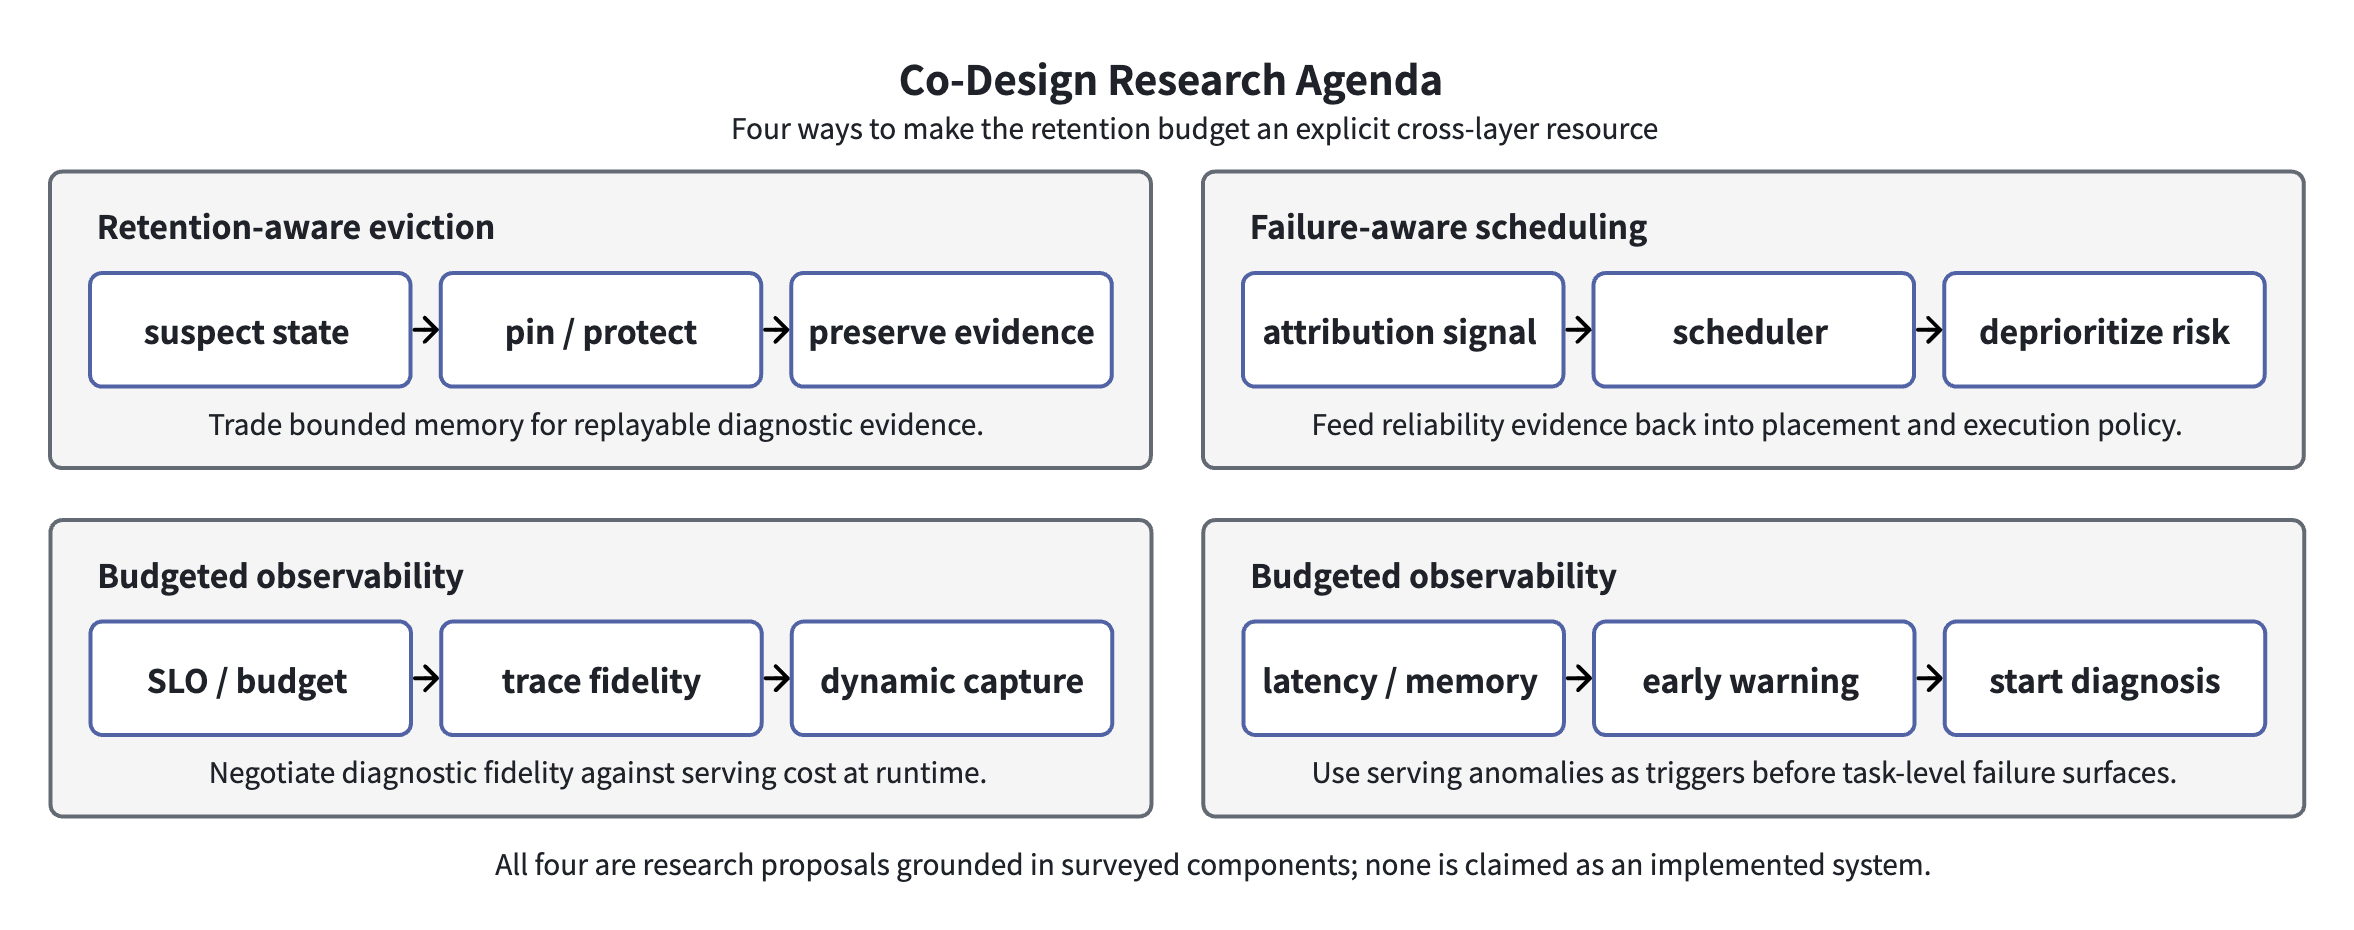
\includegraphics[width=0.9\textwidth]{figure6.png}
\caption{Co-design research agenda derived from the diagnostics--infrastructure tension. The four directions translate the tension dimensions summarized in Table~\ref{tab:tension} into testable research questions at the boundary between the two layers.}
\label{fig:codesign}
\end{figure*}

\paragraph*{Future development.}
\emph{Retention-aware eviction} targets the retention-horizon and eviction-criterion dimensions in Table~\ref{tab:tension}. A serving policy could preserve state that an online detector marks as diagnostically valuable even when predicted reuse is low, then evaluate whether the additional memory cost improves later attribution or repair.

\emph{Failure-aware scheduling} extends the runtime-state and granularity dimensions by feeding reliability evidence back into placement or execution priority. A useful evaluation would compare latency and throughput against failure containment or recovery under the same workload, rather than reporting either systems efficiency or diagnostic quality alone.

\emph{Budgeted observability} directly addresses the granularity and overhead-budget dimensions. Instead of fixing trace fidelity at design time, the system would vary capture detail under an explicit serving SLO and test whether adaptive capture preserves diagnostic accuracy more efficiently than uniform logging.

\emph{Infrastructure-triggered diagnostics} uses serving-side anomalies---for example latency spikes, memory pressure, or repeated cache churn---as early-warning signals for diagnosis. Its value would be measured by whether earlier intervention improves reliability enough to justify continuous monitoring cost. Across all four directions, the common requirement is to report the joint reliability--efficiency frontier under a shared workload and budget rather than optimize one side of the trade-off in isolation.


\section{Conclusion}\label{sec:conclusion}
Foundation model-based multi-agent systems increasingly depend on two operational layers that have largely developed apart: diagnostics, which explains and constrains failures, and infrastructure, which keeps execution efficient. This review brings them into one runtime-stack view, organizing diagnostics into failure localization, observability, safety, and benchmarks, and infrastructure into memory optimization, prefix-aware scheduling, cache lifecycle, and power management. The purpose is not to construct a leaderboard across heterogeneous systems, but to expose which assumptions each layer makes about runtime state.

The main synthesis is that diagnostics and infrastructure act on overlapping runtime objects under different objectives. Diagnostics benefits from preserving traces, context, and replayable state; serving infrastructure benefits from reclaiming or compressing state under resource budgets. The surveyed evidence makes this retention tension concrete through eviction, snapshot availability, trace compression, and replay cost, with TraceElephant providing a measured example of the sensitivity of attribution to observability. No surveyed system currently manages diagnostic value and serving value through a shared retention budget. Treating retention as an explicit cross-layer resource therefore defines a concrete research program rather than a settled result.

For future work, the most important methodological step is to evaluate reliability and efficiency jointly. Retention policies should be compared under a common workload using diagnostic fidelity, retained-state volume, serving overhead, and replay/recomputation cost. Such evaluation would make it possible to test whether retention-aware eviction, failure-aware scheduling, budgeted observability, and infrastructure-triggered diagnostics improve the joint reliability--efficiency frontier. In this sense, the contribution of the review is not only a taxonomy of recent systems, but a systems-level abstraction and validation agenda for the next generation of foundation-model multi-agent runtimes.


\fontsize{8.5pt}{10pt}\selectfont
\section*{Acknowledgements}
The authors acknowledge the use of AI-assisted tools for language editing and manuscript preparation. All technical claims, interpretations, citations, and conclusions were reviewed and remain the responsibility of the authors.

\section*{Competing interests}
The authors declare that they have no competing interests or financial conflicts to disclose.

\bibliographystyle{fcs}
\bibliography{references}

\end{document}
